\documentclass[UTF8]{ctexart}
\usepackage{amsmath,wrapfig,picinpar,graphicx}
\newcommand{\lt}{<}
\newcommand{\gt}{>}
\begin{document}
\thispagestyle{empty}
\pagestyle{empty}

\noindent 7. 设 $a=0.1e^{0.1}$,$b=\dfrac{1}{9}$,$c=-\ln 0.9$,则

\noindent A. $a \lt b \lt c$ \,
B. $c \lt b \lt a$ \,
C. $c \lt a \lt b$ \,
D. $a \lt c \lt b$ \\

\noindent 解:本题使用泰勒公式更加方便:

$$f(x)=\sum_{i=0}^{+\infty} \dfrac{f^{(i)}(x_0)}{i!} (x-x_0)^i$$

\noindent 对于函数 $a(x)=e^x$,可在 $x_0=0$ 处进行展开:

\begin{align*}
a(x) &= \sum_{i=0}^{+\infty} \dfrac{a^{(i)}(0)}{i!} x^i \\
&= 1+x+\dfrac{x^2}{2}+\dfrac{x^3}{6}+
\dfrac{x^4}{24}+\cdots
\end{align*}

\noindent 不妨计算到 $2$ 次方项:

$$a(0.1) \approx 1+10^{-1}+5 \times 10^{-3} \approx 1.105$$

\noindent 因此 $a \approx 0.1105$.

\noindent 对于 $b$,显然有 $b=0.\dot 1$.

\noindent 由于 $\ln x$ 在 $x_0=0$ 处无意义,因此不妨对函数 $c(x)=\ln (1-x)$ 在 $x_0=0$ 处进行展开:

\begin{align*}
c(x) &= \sum_{i=1}^{+\infty} (-\dfrac{x^i}{i}) \\
&= -(x+\dfrac{x^2}{2}+\dfrac{x^3}{3}+\cdots)
\end{align*}

\noindent 不妨计算到 $2$ 次方项:

$$c(0.1) \approx -(10^{-1}+5 \times 10^{-3})=-0.105$$

\noindent 因此 $c \approx 0.105$.

\noindent 整理得 $a \approx 0.1105$,$b \approx 0.1111$,$c \approx 0.105$.

\noindent 故 $c \lt a \lt b$,选 C.

\newpage

\noindent 8. 已知正四棱锥的侧棱长为 $l$,其各顶点都再同一球面上,若该球的体积为 $36 \pi$,且 $3 \le l \le 3 \sqrt 3$,则该正四棱锥体积的取值范围是

\noindent A. $[18,\frac{81}{4}]$ \,
B. $[\frac{27}{4},\frac{81}{4}]$ \,
C. $[\frac{27}{4},\frac{64}{3}]$ \,
D. $[18,27]$ \\

\noindent 解:设四棱锥底面边长为 $\sqrt 2a$,则

$$(3+\sqrt{9-a^2})^2+a^2=l^2$$

\noindent 化简得

$$a^2=\frac{36l^2-l^4}{36}$$

\noindent 设 $t=l^2$,棱锥体积为 $V(t)$,则

\begin{align*}
V(t) &= 2a^2+\frac{2a^2}{3} \times \sqrt{9-a^2} \\
&= \frac{t^2}{324}(36-t) \qquad  \qquad (t \in [9,27])
\end{align*}

\noindent 对上式求导得

\begin{align*}
V'(t) &= \frac{1}{324} \times [2t \times (36-t)-t^2] \\ 
&= \frac{24t-t^2}{108}
\end{align*}

\noindent 设能让 $V(t)$ 取极值的自变量为 $t_0$,则

$$24t_0-t_0^2=0 \Rightarrow t_0=0 \text{(舍)或 } t_0=24$$

\noindent 由此可知 $V(t)$ 在 $(9,24)$ 上为增函数,在 $(24,27)$ 上为减函数.

\noindent 因而

$$V_{\max}=V(24)=\frac{24^2}{324}(36-24)=\frac{64}{3}$$

$$V_{\min}=\min\{V(9),V(27)\}=\min\{\frac{9^2}{324}(36-9),\frac{27^2}{324}(36-27)\}=\frac{27}{4}$$

\noindent 故选 C.

\newpage

\noindent 18. 记 $\triangle ABC$ 的内角 $A,B,C$ 的对边分别为 $a,b,c$. 已知 $\dfrac{\cos A}{1+\sin A}=\dfrac{\sin 2B}{1+\cos 2B}$.

\noindent (1) 若 $C=\dfrac{2 \pi}{3}$,求 $B$. \\

\noindent (2) 求 $\dfrac{a^2+b^2}{c^2}$ 的最小值. \\

\noindent 解:化简题中条件

\begin{align*}
\dfrac{\cos A}{1+\sin A} &= \dfrac{\sin 2B}{1+\cos 2B} \\
2 \sin B \cos B(1+ \sin A) &= 2 \cos A \cos ^2 B
\end{align*}

\noindent 这里需讨论 $\cos B$ 是否为 $0$. 当 $\cos B=0$ 即 $B=\dfrac{\pi}{2}$ 时,上述等式成立.

\noindent 当 $\cos B \neq 0$ 时

\begin{align*}
2 \sin B(1+ \sin A) &= 2 \cos A \cos B \\
2(\cos A \cos B-\sin A \sin B) &= 2 \sin B \\
2 \cos(A+B) &= 2 \sin B \\
\sin B+\cos C=0
\end{align*}

\noindent 综上,$B=\dfrac{\pi}{2}$ 或 $\sin B+\cos C=0$. \\

\noindent (1) 因为 $C=\dfrac{2 \pi}{3} \gt \dfrac{\pi}{2}$,所以 $B \lt \dfrac{\pi}{2}$,因此只能有 $\sin B=-\cos C=\cos \dfrac{\pi}{3}=\dfrac{1}{2}$. \\

\noindent 故 $B=\dfrac{\pi}{6}$. \\

\noindent (2) 分类讨论:

\noindent ① 当 $B=\dfrac{\pi}{2}$ 时,原式 $=\dfrac{2a^2+c^2}{c^2} \gt 1$. \\

\noindent ② 当 $B \lt \dfrac{\pi}{2}$ 时:

\begin{align*}
\sin A &= \sin(B+C)=\sin B \cos C+\sin C \cos B \\
&= -\sin^2 B+\sqrt{(1-\cos^2 C)(1-\sin^2 B)} \\
&= 1-2 \sin^2 B \\
&= 1-2 \cos^2 C \\
\end{align*}

\noindent 因而

\begin{align*}
\dfrac{a^2+b^2}{c^2} &= \dfrac{(1-2 \cos^2 C)^2+\cos^2 C}{\sin^2 C} \\
&= \dfrac{1-4 \cos^2 C+4 \cos^4 C+\cos^2 C}{\sin^2 C} \\
&= -4 \cos^2 C-1+\dfrac{2}{1-\cos ^2 C} \\
&= 4-4 \cos^2 C+\dfrac{2}{1-\cos^2 C} -5 \\
&= 4 \sin^2 C+\dfrac{2}{\sin^2 C}-5 \\
&\ge 2 \sqrt{4 \times 2}-5 \\
&= 4 \sqrt{2}-5
\end{align*}

\noindent 当且仅当 $\sin^4 C=\dfrac{1}{2}$ 时,上式成立. \\

\noindent 则当 $B \lt \dfrac{\pi}{2}$ 时,$\dfrac{a^2+b^2}{c^2}$ 的最小值为 $4 \sqrt 2-5$.

\noindent 因为 $4 \sqrt 2-5 \lt 1$,所以 $\dfrac{a^2+b^2}{c^2}$ 的最小值为 $4 \sqrt 2-5$.

\newpage

\noindent 19. 如图,直三棱柱 $ABC-A_1B_1C_1$ 的体积为 $4$,$\triangle A_1BC$ 的面积为 $2 \sqrt 2$.

\begin{wrapfigure}{r}{5em}
	\begin{center}
	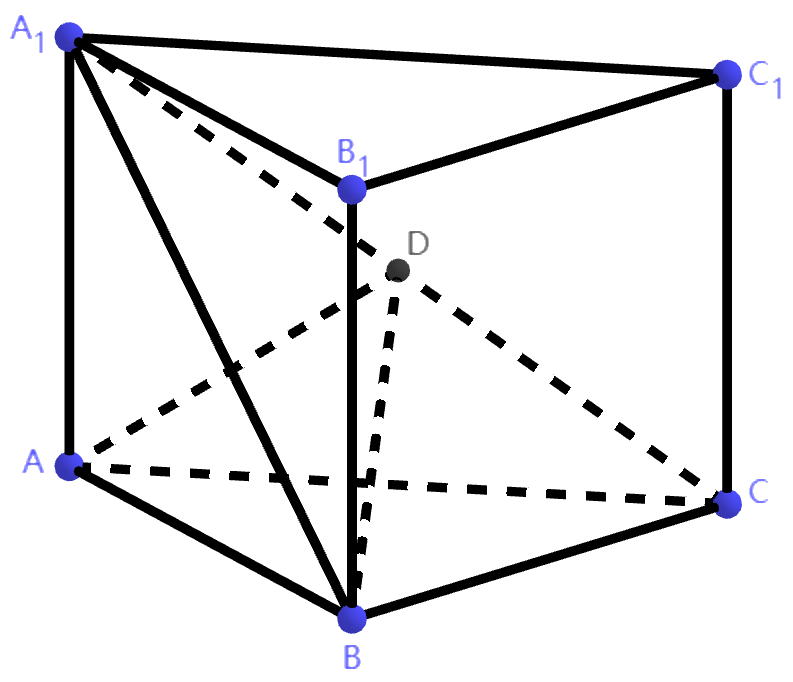
\includegraphics[width=0.5\textwidth]{19/T19-1.png}
	\end{center}
\end{wrapfigure}

\noindent (1) 求 $A$ 到平面 $A_1BC$ 的距离.

\noindent (2) 设 $D$ 为 $A_1C$ 的中点,$AA_1=AB$,平面 $A_1BC \perp ABB_1A_1$,求二面角 $A-BD-C$ 的正弦值. \\

\noindent 解:(1) $V_{A_1-ABC}=\dfrac{1}{3}V_{ABC-A_1B_1C_1}=\dfrac{4}{3}$. \\

\noindent 则 $h_{A-A_1BC}=\dfrac{3V_{A-A_1BC}}{S_{\triangle A_1BC}}=\dfrac{3V_{A_1-ABC}}{S_{\triangle A_1BC}}=\dfrac{3 \times \frac{4}{3}}{2 \sqrt 2}=\sqrt 2$.

\noindent 故 $A$ 到平面 $A_1BC$ 的距离为 $\sqrt 2$. \\

\noindent (2) 取 $A_1B$ 中点 $E$.

$$\left.
	\begin{array}{rr}
	\noindent AA_1=AB \Rightarrow A_1ABB_1 \text{ 为正方形} \Rightarrow AE \perp A_1B \\
	\text{平面 } A_1BC \cap \text{平面 } ABB_1A_1=A_1B \\
	\text{平面 } A_1BC \perp \text{平面 } ABB_1A_1
	\end{array}
\right\}
\Rightarrow AE \perp \text{平面 }A_1BC.
$$

\begin{wrapfigure}{r}{5em}
	\begin{center}
	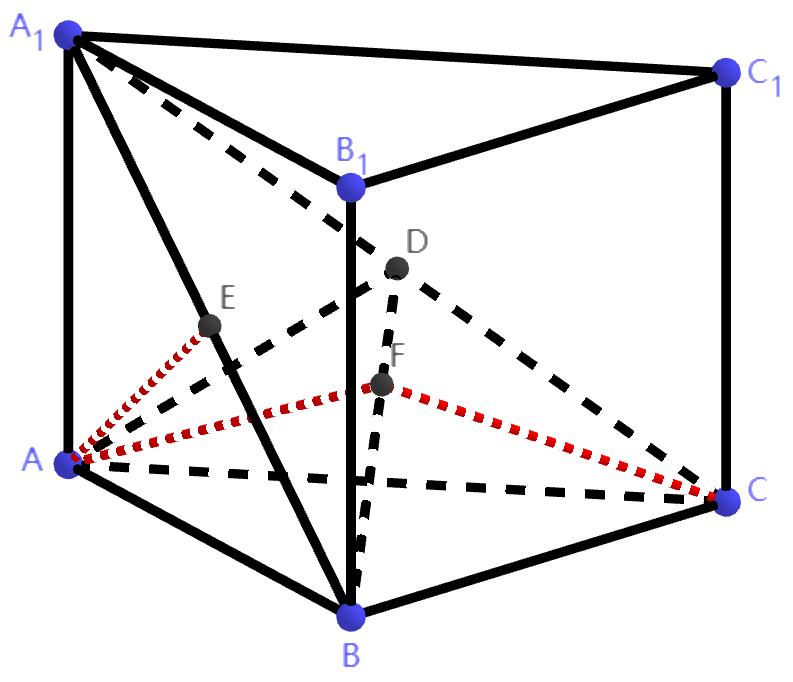
\includegraphics[width=0.5\textwidth]{19/T19-2.png}
	\end{center}
\end{wrapfigure}

\noindent 又因为 $A$ 到平面 $A_1BC$ 的距离为 $\sqrt 2$,所以 $AE=\sqrt 2 \\
\noindent  \Rightarrow A_1B=2AE=2 \sqrt 2 \Rightarrow S_{\triangle ABC}=\dfrac{V_{ABC-A_1B_1C_1}}{AA_1}=\dfrac{4}{2}=2 \Rightarrow BC=2$.

\noindent 作 $AF \perp BD$ 于 $F$. 则 $\cos \angle ABD=\dfrac{4}{4 \sqrt 3}=\dfrac{\sqrt 3}{3} \Rightarrow BF=\dfrac{2}{3} \sqrt 3, AF=2 \sqrt{\dfrac{2}{3}}=\dfrac{2}{3} \sqrt 6$. \\

\noindent 因为 $\triangle ABD$ 全等于 $\triangle CBD$,所以 $CF \perp BD$. 则 $\sin \angle AFC$ 即为所求.

\noindent 根据余弦定理

$$\cos \angle AFC=\dfrac{AF^2+CF^2-AC^2}{AC^2}=\dfrac{\frac{8}{3}+\frac{8}{3}-8}{2 \times (\frac{2}{6} \sqrt 3)^2}=-\dfrac{1}{2}$$ \\

\noindent 故二面角 $A-BD-C$ 的正弦值为 $\sqrt{1-(-\dfrac{1}{2})^2}=\dfrac{\sqrt 3}{2}$.

\end{document}